\documentclass[11pt]{article}
\usepackage[utf8]{inputenc}
\usepackage{graphicx}
\usepackage[italian]{babel}
\usepackage{hyperref}
\usepackage{float}
\title{Progetto di Tecnologie Web}


\begin{document}
	\maketitle
	\begin{figure}[h]
		\centering
		
\includegraphics[width=0.7\linewidth]{logo-unipd.png}
	\end{figure}
	\begin{center}{\fontsize{20}{10}\selectfont Autori:}\end{center}
	\begin{center}{\fontsize{20}{30}\selectfont 
			Marco Casagrande
			\\ Walter Sandon 1009138
			
			}\end{center}
	
	\newpage
	\tableofcontents
	\newpage
	\listoffigures
	\newpage
	
	\section{Abstract}
	
Il progetto sviluppato implementa il sito internet di una azienda che produce per conto terzi griglie metalliche ad uso domestico, quali griglie per forni e frigoriferi.
Il sito si propone di dare ogni informazione che possa essere rilevante agli utenti visitatori come i prodotti che la IMAS riesce a realizzare e le relative lavorazioni disponibili, la posizione della ditta  e la possibilità, nel caso si abbia la necessità di ulteriori delucidazioni, di potere contattere gli opratori tramite apposito form nell'area dedicata.
Inoltre gli amministratori hanno la possibilità di accedere ad un area riservata dalla quale modificare  o aggiungere i prodotti e lavorazioni in catalogo; in particolare lato prodotti:
\begin{itemize}
	\item inserire nuovo prodotto,
	\item assegnare a più prodotti una lavorazione, 
	\item modificare un prodotto esistente, in particolare:	
	\begin{itemize}
		\item nome
		\item foto
		\item attributo alt della foto
		\item lavorazione
		\item descrizione
	\end{itemize}
	\item eliminare un prodotto.
\end{itemize}
La lavorazione è similare al prodotto in quanto di possono eseguire le stesse operazioni di inserimento e modifica dei propri campi

\subsection{Combinazione dei colori}
Per cercare di garantire una totale usabilità del sito anche ad utenti affetti da problemi visivi è stato scelto di utilizzare uno schema a colori che esaltasse il contrasto tra sfondo e testo. Per testare tale scelta è stato utilizzato il servizio offerto da \href{http://colorfilter.wickline.org/}{\textit{wickline}} che mostra come il sito può venire visualizzato da utenti con determinati problemi. Di seguito vengono riportati i risultati ottenuti.
\newpage
\section{Utenti destinatari}
\paragraph{Privati/Aziende}
Una prima categoria di utenti destinatari del sito comprende in piccola misura i privati cittadini e nella maggioranza alle aziende che producono oggetti che rientrano nelle categorie merciologiche presenti nella sezione  \textit{Prodotti}.\\
Questi utenti potranno visualizzare il catalogo e constatare la presenza di un particolare prodotto; per questo, oltre alle informazioni di base del prodotto, si può trovare l'indicazione circa le possibili \textit{lavorazioni}.\\
Oltre a ciò, gli utenti potranno (nelle due pagine \textit{Home} e \textit{Contatti}) scoprire la storia della compagnia e qual'ora fossero interessati, chiedere informazioni tramite un apposito form.

\paragraph{Amministratori}
Un'altra categoria di utenti del sito è rappresentata dagli amministratori IMAS che potranno accedere, autenticandosi attraverso un link nell' \textit{header} a destra del logo aziendale, ad un'area riservata dalla quale è possibile gestire il catalogo dei prodotti e lavorazioni che può offrire la ditta.

\newpage

\section{Usabilità}

Dopo aver discusso col proponente riguardo alle possibili implementazioni del sito, in fase di progettazione ci siamo chiesti come distribuire le varie informazioni nel sito cercando di dare una giusta collocazione alle cose ponendo l'attenzione su due variabli quali le azioni che un utente maggiormente esegue e la tipologia aziendale in questione

\begin{description}
	\item [Consultare il catalogo prodotti] \hfill \\
	L'operazione più frequentemente compiuta dagli utenti è quella di consultare il catalogo dei prodotti presenti.
	\\
	Essendo però una ditta che non ha una continuità di rinnovo dei prodotti, si è ritenuto apportuno non metterlo in evidenza nella \textit{homepage}, ma piuttosto  dedicare un area apposita. 
	La \textbf{Home} è stata adibita a chi entra per la prima volta nel sito o piuttosto qualche vecchio utente che vogliano informarsi circa sulle origini, sulla storia o sulla mission aziendale. \\
	Nel contempo in queste sezioni sono stati inseriti link diretti per poter consultare i nostri prodotti  ed è stata inoltre predisposta una comoda \textit{NavBar} con la quale raggiungere comodamente le pagine \textbf{Prodotti} e \textbf{Lavorazioni}, i cui nomi sono esplicativi circa le informazioni contenute.
	Stessa considerazione va fatta per la \textbf{consultazione delle lavorazioni}.

	\item [Manutenzione del catalogo] \hfill \\
	L'operazione di manutenzione dei cataloghi (aggiunta, modifica e rimozione dei prodotti/lavorazioni) è riservata agli amministratori del sito.\\
	 È logico pensare che, essendo tali utenti un numero inferiore rispetto ai visitatori, il link per l'autenticazione e l'accesso all'area riservata possa essere messa in posizione \textit{nascosta}. Portroppo per ragioni di spazio l'abbiamo posizionata solo in alto a destra sapendo di creare così disorientamento.\\
	 Abbiamo cercato di limitare i danni avvisando,  una volta entrati nell'area login, che tale area è riservata ai dependenti IMAS.\\
	  \textit{Si noti che il pulsante per poter entrare nell'area gestione prodotti e lavorazioni è visibile solo quando  l'amministratore ha eseguito il login.}
\end{description}
\subsection{Elementi dell'Interfaccia Grafica}

Analizziamo ora gli elementi dell'interfaccia utilizzati per renderla il più chiara (intuitiva per ogni utente) e diretta (minor numero di click per un operazione) possibile.
\begin{description}
	\item [NavBar] La barra di navigazione è presente in ogni pagina e consente l'accesso diretto alla homepage, l'accesso alle pagine \textit{Prodotti}, \textit{Lavorazioni} e \textit{Contatti}.
	\\È stata progettata in modo tale che l'utente sappia in ogni momento in che pagina si trova. Infatti la parte della barra corrispondente alla pagina visitata risulta essere evidenziata.
	\item [Breadcrumbs] Per evitare che l'utente si senta disorientato all'interno del sito, quando dalla homepage si addentra con maggiore profondità nella struttura del sito, compare il percorso dell'utente a partire dalla homepage.
	\item [Link] Abbiamo deciso di adottare due tipologie di link, quelli che si trovano immersi nel testo e quelli che invece sono inseriti nelle due sezioni precedentemente descritte.
	\\ I primi sono sottolineati e aderiscono alla rappresentazione standard dei link ovvero blu se non visitati e viola in caso contrario.Tutti gli altri inseriti nelle sezioni \textit{nav bar} e \textit{Breadcrumbs} sono comunque ben visibili con il passaggio del mouse grazie all'effetto \textbf{hover}.
\end{description}

\newpage
\section{Gerarchia file}

La gerarchia del sito è formata da 3 cartelle:
\begin{itemize}
	\item \texttt{cgi-bin} con gli script \texttt{.cgi}
	\item \texttt{data} con 3 sotto-cartelle
	\begin{itemize}
		\item \texttt{xml} contente tutti i file xml
		\item \texttt{xsd} contente gli \textit{XMLSchema}
		\item \texttt{xsl} contenete i fogli di trasformazione
	\end{itemize}
	\item \texttt{public\_html} con il file \texttt{index.xhtml} e le sotto-cartelle:
	\begin{itemize}
		\item \texttt{images} con le immagini che ci sono servite per decorare il sito
		\item \texttt{icons} con l'e icone per i tab dei browser
		\item \texttt{javascript} con le funzioni appunto in \textit{JavaScript}
		\item \texttt{parts} con i file xhtml parziali, ovvero parti di codice xhtml che verranno stampate dinamicamente grazie al perl
		\item \texttt{css} con i fogli di stile  
	\end{itemize}
\end{itemize}
\newpage
\section{Architettura}
\subsection{Progettazione layout}
Prima di iniziare la stesura del codice abbiamo cercato di organizzare i dati che volevamo rappresentare. Questo ci ha permesso di chiarire alcuni aspetti fondamentali che il sito doveva avere. Innanzitutto la semplicità di navigazione al suo interno. Se un sito è semplice è visitabile e capibile da più persone. Il target d'utenza è l'utente in grado di utilizzare strumenti per la navigazione sul web.
\\
\\
Fin da subito abbiamo optato per un layout di tipo fluido. Ha richiesto più lavoro del previsto ma ha ricompensato lo sforzo in quanto, abbiamo dovuto adattarlo ai vari tipi di monitor cambiando di molto l'aspetto, ma questo ha reso possibile un alto indice di accessibilità.
\subsection{Sviluppo layout}
Nell'immagine sottostante è possibile visualizzare la struttura principale dei div, i quali raccolgono per contenuto tematico le informazioni.
Il layout adottato ha come larghezza massima 1200px dovuto ad un fattore estetico dato che le varie sezioni del \textit{Container} cambia di colore ad ogni cambio d'informazione, mentre l'altezza non è stata in nessun modo alterata rispetto l'originale. Questo permette una evoluzione verso il basso senza problemi.
\begin{figure}[H]	
	\centering
	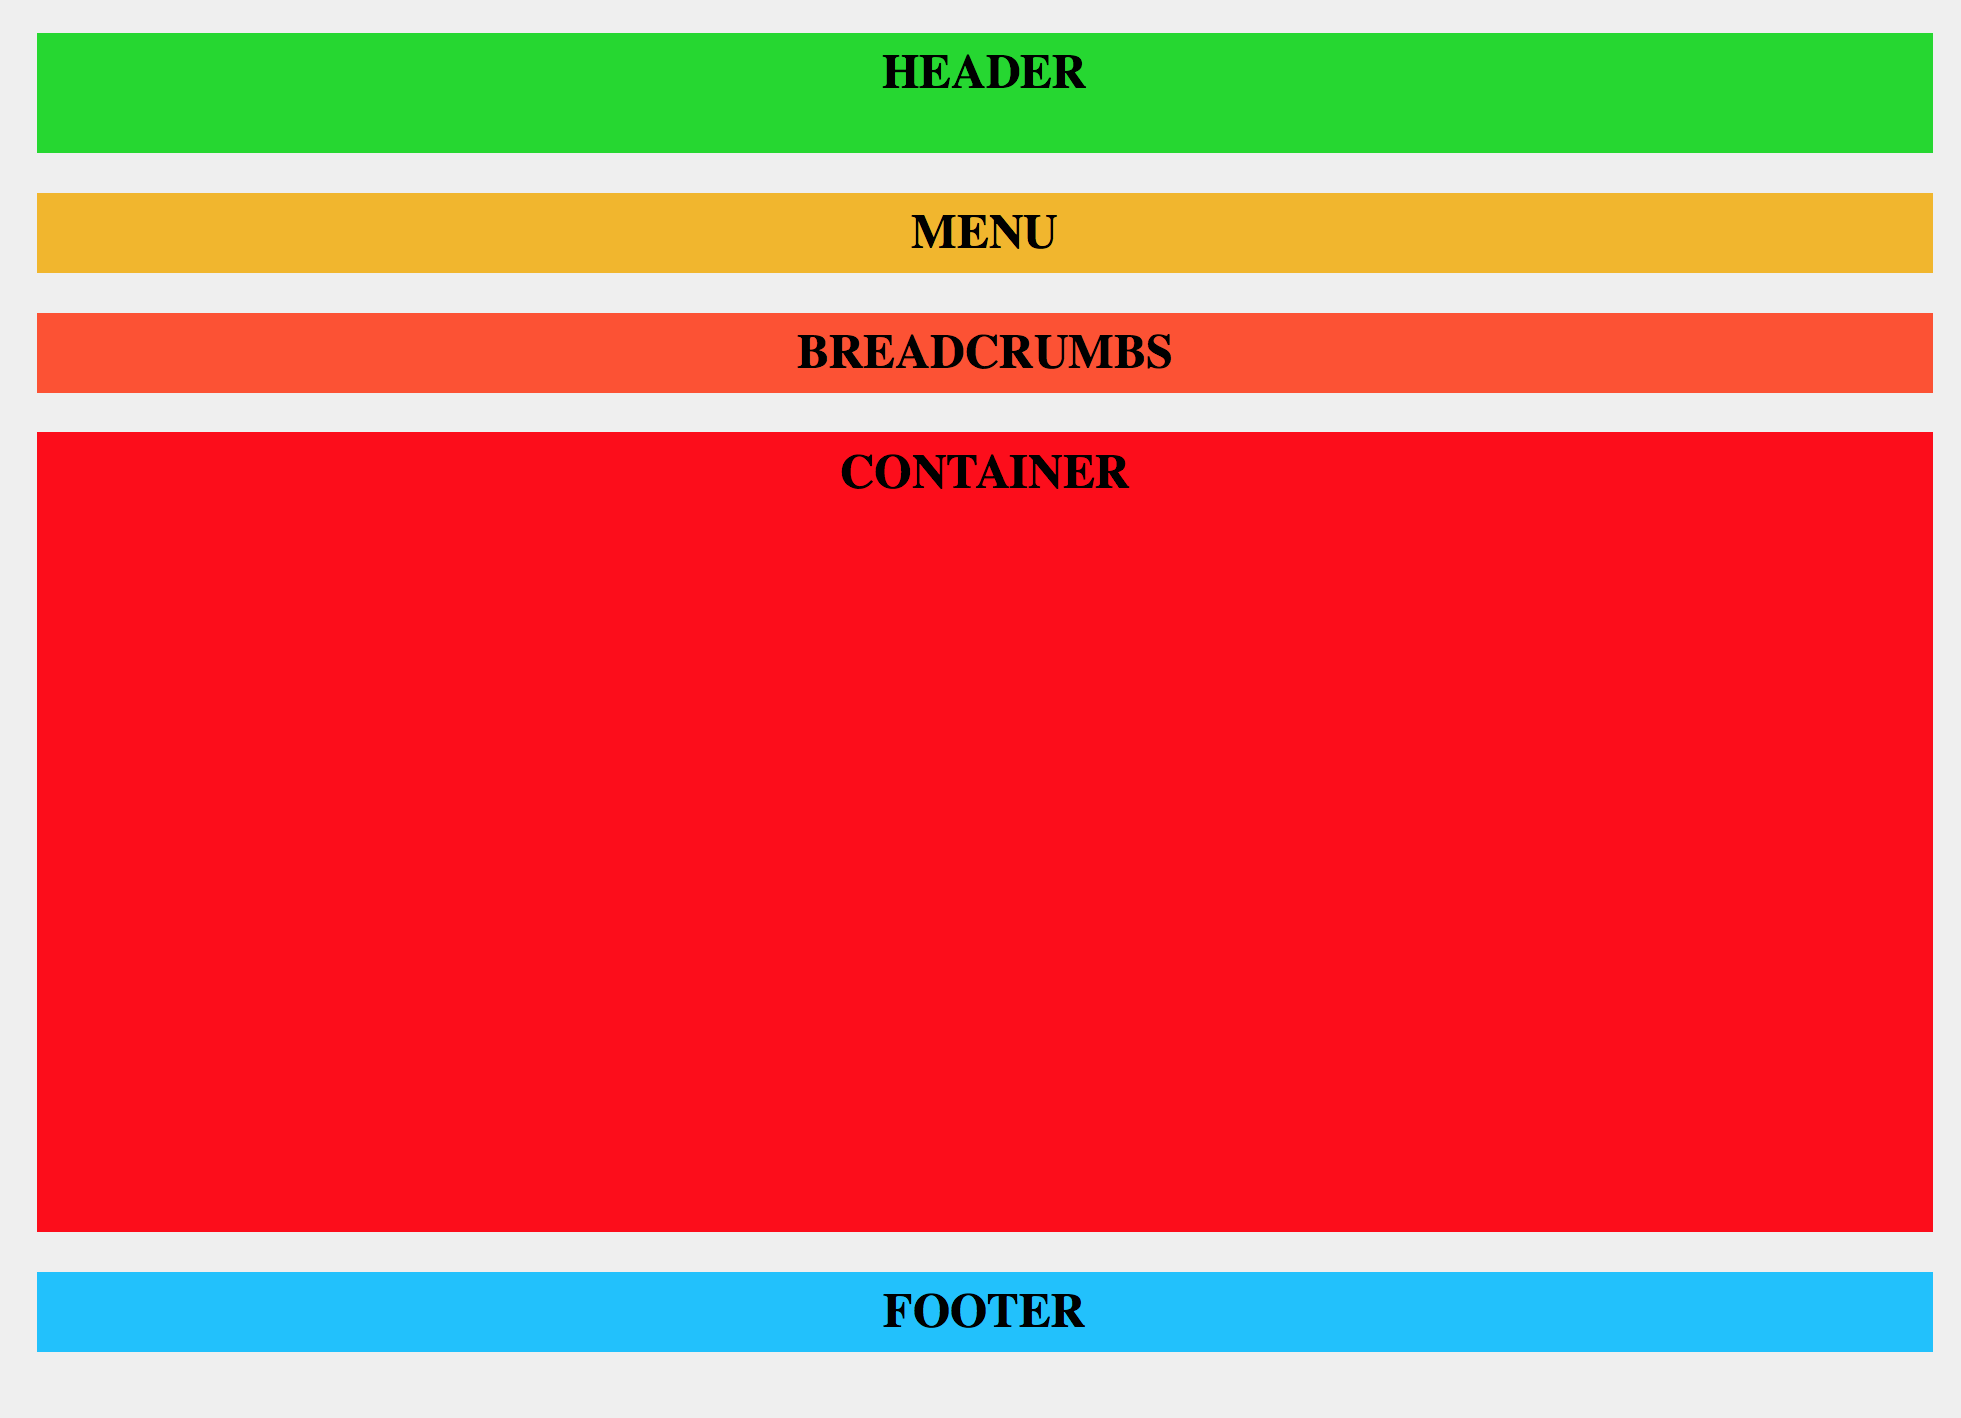
\includegraphics[width=\linewidth]{layout.png}
	\caption{Layout delle pagine}
	\label{Layout delle pagine}
\end{figure}

Per quanto riguarda il nostro contesto, la maggioranza degli utenti visitatori saranno aziende interessate alla nostra ditta pertanto si è deciso di puntare ad un layout adatto a partatili piuttosto che a schermi di grandi dimensioni. Non abbiamo sviluppato la parte mobile lato smartphone garantendo comunque che i contenuti non subiranno alterazioni spiacevoli fino a quando la grandezza dello schermo sarà grande come i table in modalità portrait. 
\\
\\
Tutto il layout è stato progettato a pannelli adattabili, in questo modo si ha una più espandibilità.
\begin{itemize}
	\item Partendo con l'analisi dall'alto si evidenzia subito il div "header", esso ha il compito di informare l'utente su ciò che sta visitando.
	\\In questo caso siamo stati un pò condizionati dal fatto che non avevamo una totale libertà. Infatti manca una breve descrizione per far capire all'utent quale sia la tematica del sito.
	\\Come spiegato in precedenza a lato a destra è presente il link per l'accesso agli amministratori.
	\item Sempre nell'area di maggior visibilita è presente il menu utente. Anch'esso è stato identificato tramite l'utilizzo del div "menu". Presenta 4 campi rappresentati da \textbf{Home}, \textbf{Prodotti}, \textbf{Lavorazioni} e \textbf{Contatti}. Evidenzia il menù attivo in ogni pagina del sito. Questa area rappresenta l'asse informativo di dove un utente può andare.
	\item Sottostante il menu principale è presente il div "breadcrumbs". Esso ha il compito di aiutare l'utente ad identificare in che posizione del sito si trova rispetto l’homepage del sito. Questa area rappresenta l'asse informativo di dove l'utente sia in quel determinato istante.
	\item Il blocco centrale è rappresentato dal div "container". Ha il compito di raccogliere la sezione principale, tutte le informazioni raccolte dagli utenti verranno rappresentate all'intero di esso. Questa area rappresenta l'asse informativo di cosa si sta trattando.
	\item Nella parte inferiore del sito è stato creato il div "footer", al suo interno sono presenti le credenziali della ditta e i loghi della certificazione html e css.
\end{itemize}

\subsection{Layout per dispositivi mobili}
Il layout per i dispositivi mobili è stato sviluppato per risoluzioni non inferiori ai 768px, l'aspetto del sito non varia, ma si è cercato di ridimensionare le dimensioni dei font piuttosto che la grandezza delle immagine in modo da utilizzare quanta più area possibile per la visualizzazione.
\\Ove non è stato possibile abbiamo cambiato la disposizione degli oggetti.

\subsection{Layout di stampa}
Nel layout di stampa si è deciso di eliminare tutte le informazioni superficiali e di mantenere il contenuto semplice e privo di colori e immagini. Anche in questa parte i font non sono stati modificati rispetto a quelli di default, in modo da non alterare la relativa qualità di stampa o portabilità nel caso di stampa in PDF.
\newpage
\section{Struttura}
\newpage

\section{Presentazione}
\newpage
\section{Comportamento}
\newpage
\section{Gestione dati}
\newpage
\section{Perl}
\newpage
\section{Validazione}
\end{document}
